\chapter{Strumenti fondamentali} \label{tools}
Prima di addentrarci nella trattazione del teorema, richiamiamo alcune nozioni alla base di quanto diremo più avanti. 
In particolare, avere chiare queste informazioni risulterà cruciale per assicurarsi di aver compreso a fondo il significato delle ipotesi che richiederemo e le tecniche dimostrative utilizzate.

Prima di tutto, anche per cominciare a prendere familiarità con la notazione, ripassiamo la nomenclatura delle equazioni equazioni differenziali di ordine $k$, e di conseguenza degli operatori ad esse associate, con una tabella riassuntiva:
\vspace{5mm}
\begin{center}
\renewcommand{\arraystretch}{2}
\begin{tabular}{l l} 
\hline \hline
 Lineare & $\sum_{|\alpha |\leq k} a_\alpha \, D^\alpha u = f$ \\
 \hline
 \vspace{-2mm}
 Quasi-lineare & $\sum_{|\alpha |= k} a_\alpha (x,D^\beta u) \, D^\alpha u +  a_0(x,D^\beta u)= f,$\\
 & $\quad |\beta |<k $ \\
 \hline
 Non lineare & $F(x,D^\alpha u)=0, \quad |\alpha | \leq k$ \\
 \hline
 In forma normale & $D_{t}^k u = G(x,t, D^\alpha_x D^j_t u), \quad |\alpha |+j \leq k, \, j < k$ \\
 \hline \hline
\end{tabular}
\end{center}
\vspace{5mm}
\begin{remark}
Da qui in poi non faremo sempre particolare attenzione alle assunzioni di regolarità dei dati delle equazioni ($f,a_\alpha,F,G$ e altro), poiché ai nostri scopi è sufficiente che le affermazioni siano vere nel caso in cui tutto sia assunto analitico (con un certo raggio di convergenza). Lo stesso vale per i dati e le superfici dei problemi di Cauchy associati. In ogni caso, quando non specificato, la regolarità può essere considerata come almeno $C^1$.
\end{remark}
\begin{remark}
Nel caso di equazione in forma normale si dividono le variabili tra spazio $x\in \mathbb{R}^{n-1}$ e tempo $t$, per una ragione che sarà chiara una volta conclusa la lettura di questo capitolo.
\end{remark}
Cominciamo già ad anticipare che, successivamente, i coefficienti e le funzioni che definiscono le equazioni li assumeremo molto regolari, per la precisione analitici (ovvero localmente sviluppabili in serie di potenze).
\newpage
Alla luce di quanto detto fin'ora, ci rendiamo conto di come ci sarebbero già alcuni aspetti su cui sarebbe importante soffermarsi.
Ma per essere più ordinati riassumiamo le nostre tematiche di interesse in quattro punti, i quali rispecchiano la struttura dei questo capitolo:
\begin{enumerate}
\item \textbf{superfici caratteristiche}: ovvero quelle superfici in $\mathbb{R}^n$ che sono strettamente legate alla forma dell'equazione in osservazione e che possono essere fonte di problemi quando si decide di assegnare dei dati Cauchy su di esse;
\item \textbf{metodo delle caratteristiche}: nel caso di equazioni, anche non lineari, del primo ordine è possibile vedere un'EDP come un sistema di EDO dipendente da un parametro;
\item \textbf{problemi di Cauchy}: l'unica tipologia di problemi di cui ci occuperemo;
\item \textbf{serie di potenze}: costituiscono le fondamenta del concetto di funzione analitica (e olomorfa nel caso dei numeri complessi), ovvero l'unica tipologia di funzioni che cercheremo come soluzione. 
\end{enumerate}


\section{Superfici caratteristiche} \label{supcar}
In questa prima sezione introduciamo il concetto di superficie caratteristica nei casi più semplici, in modo da comprenderne a pieno il significato. Cominciamo mettendoci nella situazione più semplice in assoluto, ovvero quella di un'equazione lineare. 
Tale equazione è univocamente determinata dal termine forzante che abbiamo chiamato $f$ e da un operatore differenziale lineare $L=\sum_{|\alpha |\leq k} a_\alpha \, D^\alpha$. Concentriamo la nostra attenzione su quest'ultimo e diamo tre definizioni.

\begin{definition}
Forma caratteristica di $L$:  $\chi_L(x,\xi)=\sum_{|\alpha |= k} a_\alpha(x) \, \xi^\alpha$ con  $x,\xi \in \mathbb{R}^n$.
\end{definition}

\begin{definition}
Varietà caratteristica di $L$ in $x$: $\text{char}_x (L)= \{ \xi \neq 0 : \chi_L(x,\xi)=0 \}$.
\end{definition}

\begin{definition} \label{supcarlin}
$\Gamma$ superficie caratteristica per $L$ in $x \iff \nu(x) \in\text{char}_x (L)$.
\end{definition}

Cerchiamo ora di indagare il significato di queste definizioni:
\begin{itemize}
\item Prima di tutto notiamo che quando $\xi \in \text{char}_x (L)$ è come se l'operatore non fosse ``propriamente'' di ordine $k$ nella direzione $\xi$.
\item Inoltre nel caso di operatore del primo ordine ($k=1$), una superficie $\Gamma$ è caratteristica quando $A=(a_1,\ldots ,a_n)$ è tangente a $\Gamma$ punto per punto (ovvero per ogni $x\in \Gamma$).
\item E' possibile dimostrare che una superficie caratteristica ``porta con sé più informazioni'' nel momento in cui si assegnano delle condizioni di Cauchy su di essa. Infatti, note le derivate normali $D^j_\nu u \,(j<k)$ di una funzione $u$ che vogliamo soddisfi l'equazione, nel caso in cui $\Gamma$ non sia caratteristica in ogni punto, è possibile calcolare tutte le derivate parziali di $u$ su $\Gamma$.
\end{itemize}
\newpage
Specialmente l'ultima considerazione, a causa della scarsa rigorosità, potrebbe essere fonte di confusione ad una prima lettura. Esiste però un teorema, che mostra tale risultato in modo esplicito nel caso di equazioni quasi-lineari e che può essere trovato insieme alla dimostrazione in \cite[cap.4.6]{Evans}.

\noindent\rule[0.5ex]{\linewidth}{0.2pt}
Considerando che ambiamo a dimostrare un teorema che si rivelerà molto generale, notiamo che, purtroppo, le equazioni lineari non saranno sufficienti a risolvere tutti i nostri problemi. Per questo motivo, vogliamo generalizzare immediatamente il concetto di superficie non caratteristica al caso quasi-lineare, anche se rimaniamo nel caso di equazione del primo ordine. Supponendo di avere il problema di Cauchy
\begin{equation}
\begin{cases}
\sum a_j(x,u)D_{x_j} u = b(x,u)\\
u = \phi \text{ su } \Gamma
\end{cases}
\end{equation}
e che $\Gamma$ abbia come parametrizzazione locale in un intorno di $x_0\in \Gamma$ la funzione $\gamma (s): \mathbb{R}^{n-1}\rightarrow \mathbb{R}^n$, forniamo la seguente generalizzazione, chiaramente ispirata al caso di operatori lineari del primo ordine.
\begin{definition}
$\Gamma$ non caratteristica in $x_0=\gamma (s_0)$ se e solo se\\
\begin{equation*}
\det
\underbrace{
\left[
\begin{matrix}
D_{s_1}\gamma_1 & \cdots & D_{s_{n-1}}\gamma_1 \\
\vdots &  & \vdots \\
D_{s_1}\gamma_n & \cdots & D_{s_{n-1}}\gamma_n \\
\end{matrix}\;\right|}_{\text{span del piano tangente}} \,
\left.
\begin{matrix}
a_1(\gamma, \phi(\gamma))\\
\vdots\\
a_n(\gamma, \phi(\gamma))\\
\end{matrix}\right] (s_0) \neq 0.
\end{equation*}
\end{definition}
Adesso è arrivato il momento di utilizzare queste definizioni per trarre qualche conseguenza utile.

\newpage
\section{Metodo delle caratteristiche}\label{metodocar}
Affrontiamo un'applicazione della nozione di superficie non caratteristica: il metodo delle caratteristiche per EDP del primo ordine. 
Esso è un metodo per trovare delle soluzioni di equazioni, eventualmente anche completamente non lineari, che si basa sull'idea di trasformare il problema in un sistema di EDO, che risulta essere equivalente. 

Partiamo direttamente dal caso di un'equazione quasi-lineare e consideriamo nuovamente il relativo problema di Cauchy con dati assegnati su una qualche superficie $\Gamma$. Vogliamo mostrare che tale problema è \textbf{equivalente} a un problema per un sistema di EDO.
\begin{align} 
\label{edpquasilin}
\text{EDP : }&
\begin{cases}
\sum a_j(x,u)D_{x_j} u = b(x,u)\\
u = \phi \text{ su } \Gamma
\end{cases} \\ 
\label{sisedo}
\text{EDO : }&
\begin{cases}
D_t \, x = A(x,y) \; \\
D_t \, y = b(x,y)\\ 
x(0)=x_0, \; y(0) = \phi (x_0) \quad \forall x_0 \in \Gamma
\end{cases} 
\end{align}
Dove $y = u(x)$ e $A(x,y)=(a_1(x,y),\ldots ,a_n(x,y))$.
\begin{remark}
E' importante sottolineare tre aspetti:
\begin{itemize}
\item le soluzioni $x$ vengono dette \textbf{curve caratteristiche};
\item il secondo problema è parametrico rispetto a $x_0$, quindi l'intera soluzione di $u$ sarà data dall'unione su tutti gli $x_0\in \Gamma$ di tutte le $y$ lungo le curve $x$;
\item il caso di equazione lineare è immediato da ricavare da quanto scritto sopra, assumendo semplicemente che i coefficienti $a_j$ dipendano solo da $x$ e che $b$ sia della forma $b(x,u)=f(x)-c(x)u$.
\end{itemize}
\end{remark}
Senza fornire un enunciato preciso procediamo facendo un ragionamento comunque rigoroso, che può essere considerato una dimostrazione dell'equivalenza.
\begin{proof}
in entrambe le direzioni una semplice derivazione di funzione composta:
\begin{enumerate}
\item Supponiamo di conoscere, per ogni $x_0$, $y(t)$ e $x(t)$ che risolvono il problema \eqref{sisedo}. Quindi per ogni $x_0$ vale che:
$$b(x,y) = D_t y = \sum D_{x_j} y \; D_t x_j = \sum a_j(x,y) D_{x_j} y.$$
Da cui segue che la funzione $u(x)$ che ha grafico dato dall'unione di tutte le curve $(x(t),y(t))$ risolve il problema \eqref{edpquasilin}.
\item Assumiamo ora invece di conoscere $u$ soluzione di \eqref{edpquasilin}. Troviamo $x$ risolvendo $\forall j$:
\begin{equation*} \label{sys}
D_t \, x_j = a_j(x,y), \quad x_j(0)=(x_0)_j 
\end{equation*}
Definiamo $y(t)=u(x(t))$ e, infine, utilizziamo lo stesso ragionamento di prima per concludere che $y$ soddisfa l'equazione del sistema di EDO:
$$D_t y = \sum D_{x_j} u \; D_t x_j = \sum  a_j(x,y)D_{x_j} u = b(x,y).$$
\qedhere
\end{enumerate}
\end{proof}
A questo punto potrebbe sorgere la curiosità di capire dove nasca l'idea di verificare l'equivalenza con quello specifico sistema di EDO. La risposta a tale quesito risulta essere interessante, perché racchiude in sé il significato geometrico di questo metodo. Infatti, ricordando che il versore normale al grafico di una funzione $u$ è proporzionale al vettore $(\nabla u , -1)$, possiamo affermare che l'equazione \eqref{edpquasilin} ci sta dicendo che il campo vettoriale seguente deve essere  \textbf{tangente} al grafico di $u$.
$$(a_1(x,u(x)),\, \ldots ,\, a_n(x,u(x)),\, b(x,u(x)))=(A(x,u(x)),\, b(x,u(x)))$$

\noindent\rule[0.5ex]{\linewidth}{0.2pt}

Compreso questo ultimo aspetto comincia già a delinearsi il ruolo della proprietà della caratteristicità di una superficie, infatti se una superficie è caratteristica il campo vettoriale appena 
Notiamo fin da ora che per i sistemi di EDO esistono teoremi che garantiscono esiste e unicità locale di soluzioni.
\begin{theorem}\label{teoescar}
\hpth{
\text{Problema \eqref{edpquasilin} } \\
a_j, \, b, \, \phi , \, \Gamma \in C^1\\
\Gamma \text{ non caratteristica}
}{
\exists ! \text{ soluzione } C^1 \text{ in un intorno di } \Gamma
}
\end{theorem}
La dimostrazione completa e dettagliata può essere trovata in \cite[cap.1]{Folland}, qui ne accenniamo solo le idee fondamentali. L'unicità seguente semplicemente dal fatto che il grafico della soluzione $u$ può essere vista come l'unione delle curve $(x(t),y(t))$, le quali non si intersecano se si prende un intorno abbastanza piccolo di $\Gamma$. Per dimostrare l'esistenza si utilizza la rappresentazione dell'equazione come un insieme parametrico di sistemi di EDO per svolgere i seguenti passi:
\begin{enumerate}
\item applicare il teorema di esistenza e unicità locale per EDO;
\item dimostrare l'invertibilità di $x(s,t)$, dove $s$ è una variabile ausiliaria legata alla parametrizzazione locale di $\Gamma$, grazie alla non-caratteristicità;
\item quindi definire in modo agevole la soluzione $u(x)$ seguendo la stessa idea del punto 1 dell'ultima dimostrazione fatta;
\item verificare con la derivazione di funzione composta che $u$ è soluzione dell'equazione.
\end{enumerate}
Sia la definizione di superficie caratteristica che il metodo delle caratteristiche possono essere generalizzati al caso di generica equazione del primo ordine. Inoltre esiste anche una generalizzazione del teorema \ref{teoescar} per il caso non lineare, identica sia in spirito che nel merito al caso quasi-lineare.
Non affronteremo in dettaglio questo argomento, in quanto non aggiunge nulla a livello di comprensione qualitativa dell'argomento e non tornerà utile nella successiva trattazione. Per approfondire si può fare riferimento a \cite[cap.1]{Folland} e \cite[cap.3]{Evans}.

La nozione di superficie non caratteristica, però, non è sufficiente ai nostri scopi e, nel prossimo paragrafo, vogliamo estenderla al caso più generale possibile: equazioni non lineari di qualsiasi ordine.

\newpage
\section{Problemi di Cauchy} \label{pb}

Fino ad ora abbiamo visto solo caso più semplice di problema di Cauchy, ovvero quello per un'equazione del primo ordine, dove è necessario assegnare solamente il valore delle funzione su una superficie. Per una equazione di un ordine qualsiasi questa informazione non è sufficiente a determinare univocamente la soluzione, infatti tipicamente quello che si fa è assegnare anche le \textbf{derivate normali} della soluzione $D^j_\nu u$ con $j<k=$ ordine dell'equazione. 

Ci sono altri due punti importanti che vanno tenuti sempre a mente quando si parla di problemi di Cauchy:
\begin{itemize}
\item spesso vengono utilizzati quando la superficie dei dati \textbf{non} è un bordo ($\neq$ problemi di Dirichlet);
\item portano con sé il rischio di essere \textbf{sovradeterminati}, ovvero sono un buon approccio per stabilire l'unicità della soluzione e lo sono meno per l'esistenza.
\end{itemize}

\noindent\rule[0.5ex]{\linewidth}{0.2pt}

Alla luce di quanto detto nei due paragrafi precedenti abbiamo già intuito che la nozione di superficie non caratteristica ci è utile per identificare quelle superfici su cui vogliamo assegnare delle condizioni di Cauchy in modo tale da avere qualche garanzia sull'esistenza della soluzione in intorno della superficie. Ora ci occupiamo di capire cosa si intende per superficie caratteristica nel caso più generale che possiamo immaginare, seguendo l'approccio più semplice e diretto possibile, in quanto non necessità di particolari dimostrazioni.
Consideriamo quindi il problema di Cauchy:
\begin{equation}
\begin{cases}
F^*(x,D^\alpha u^*)=0 & |\alpha | \leq k, \, F^*\\
D^j_\nu u^* = \phi_j^* & \text{su } \Gamma^* \text{ per }j<k 
\end{cases}
\end{equation}

A prescindere dalla forma dell'equazione è possibile modificare questo problema in modo tale da appiattire localmente il bordo della superficie rispetto a una variabile. Per ottenere questo risultato è sufficiente un semplice cambio di coordinate $\Phi$, definita tramite $\gamma^*$ (parametrizzazione locale di $\Gamma^*$):
$$\Phi (x) = 
\left( \begin{matrix}[ccc|c]
x_1 & \cdots & x_{n-1} & x_n-\gamma^* (x_1,\ldots , x_{n-1})
\end{matrix}\right)$$
\begin{figure}[H]
\centering
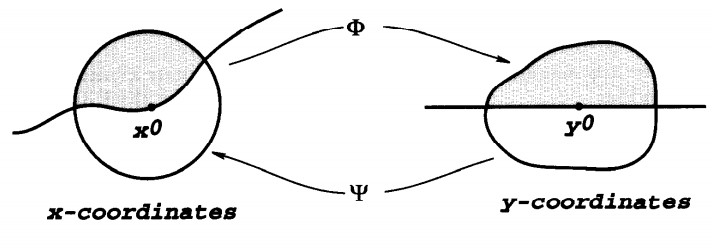
\includegraphics[scale=.5]{flatb}
\caption{Immagine da \cite[cap.8]{Evans}}
\end{figure}
\begin{remark}
Notiamo che $\Phi$ preserva l'eventuale analiticità della superficie $\Gamma^*$.
\end{remark}

Questa trasformazione ci fa capire come sia possibile scegliere di considerare  ``privilegiata''. Da qui in poi essa prenderà il nome di ``tempo'' e la indicheremo con la lettera $t$. Per essere più precisi rinominiamo le variabili nel modo seguente:
\begin{align*}
t & \leftarrow x_n \\
x & \leftarrow (x_1,\ldots , x_{n-1})
\end{align*}
Inoltre, introduciamo un po' di notazione che tornerà utile più avanti:
\begin{itemize}
\item chiamiamo $\Gamma_0 = \{t=0\}$.
\item indichiamo le derivate nel modo seguente: $D^\alpha_x D^j_t u$.
\end{itemize}
Concludiamo quindi che grazie alla trasformazione $\Phi$ otteniamo il nuovo problema:
\begin{equation}\label{gamma0prob}
\begin{cases}
F(x,t, D^\alpha_x D^j_t u)=0 & |\alpha | +j \leq k\\
D^j_t u (x,0)= \phi_j(x) & \text{per }j<k 
\end{cases}
\end{equation}
dove $u^*=u(\Phi)$.

\noindent\rule[0.5ex]{\linewidth}{0.2pt}

\begin{definition}
$\Gamma^*$ (o $\Gamma_0$) è non caratteristica se l'equazione su $\Gamma_0$ può essere riscritta in \textbf{forma normale} rispetto a $t$, ovvero se il problema \eqref{gamma0prob} può essere riscritto così:
\begin{equation*}
\begin{cases}
D_{t}^k u = G(x,t, D^\alpha_x D^j_t u) & |\alpha |+ j \leq k, \, j<k \\
D_t^ju = \phi_j & \text{ su } \Gamma_0, \, j<k
\end{cases} \\
\end{equation*}
\end{definition}

Per rendere più concreta questa definizione spesso si cercano delle condizioni sufficienti, ed eventualmente anche necessarie, perché l'equazione possa essere riscritta in forma normale, come abbiamo fatto noi nel paragrafo \ref{supcar} per i casi più semplici e come è stato fatto in \cite{Evans} e in \cite{Folland}.
Vediamo quindi di cosa si tratta, distinguendo i vari casi e ipotizzando di esserci già messi nella situazione \eqref{gamma0prob}:
\begin{itemize}
\item lineare e quasi-lineare: si richiede che $a_{(0,\ldots ,0,k)} \neq 0$ su $\Gamma_0$;
\item non lineare: si richiede la validità ipotesi teorema della funzione implicita (noto anche come teorema del Dini) su $F$, ovvero $D_{(D^k_t u)} F \neq 0$ su $\Gamma_0$.
\end{itemize}

\begin{remark}
Sempre rimanendo nell'ipotesi che la superficie sia $\Gamma_0$, a partire da queste considerazioni è facile vedere come la nuova definizione di superficie non caratteristica sia coerente con le definizioni del paragrafo \ref{supcar}.
\end{remark}

Ricordiamo, infine, che la nozione di superficie caratteristica ci deve garantire la possibilità di calcolare tutte le derivate parziali della soluzione sulla superficie. Per questa ragione l'impostazione di questa costruzione si ispira, in parte, a \cite[cap.3]{Evans}, dove è presente la dimostrazione di questa proprietà in due passi:
\begin{enumerate}
\item prima si ragiona ipotizzando di essere su $\Gamma_0$;
\item grazie alla trasformazione $\Phi$ si ottiene la proprietà per una generica $\Gamma^*$.
\end{enumerate}


\newpage
\section{Serie di potenze}\label{seriedipotenze}
Dando per nota la teoria delle funzioni olomorfe, e di conseguenza anche la teoria base delle funzioni analitiche (reali), in questo paragrafo vogliamo scoprire, o conoscere meglio, solamente degli strumenti molto specifici che ci permetteranno di dimostrare il TCK.

Cominciamo con lo studiare uno sviluppo in serie di potenze di una funzione di cui non dobbiamo dimenticarci.
\begin{definition}
Funzione maggiorante: $$\mathcal{M}_{Cr}(x)=\frac{Cr}{r-(x_1+\ldots +x_n)}$$
\end{definition}
Utilizzando il teorema multinomiale, dimostriamo che la questa funzione può essere sviluppata in serie di potenze per $|x|<r/n$, ricavandone l'espressione dei coefficienti $c_\alpha$:
\begin{align*}
\mathcal{M}_{Cr}(x) &= \frac{Cr}{r-(x_1+\ldots +x_n)} = C \sum\limits_{j=0}^\infty \left(\frac{x_1+\ldots +x_n}{r}\right)^j  \\
&= C \sum\limits_{j=0}^\infty \frac{1}{r^j} \sum\limits_\alpha  \binom{|\alpha |}{\alpha } x^\alpha = \sum\limits_\alpha 
\underbrace{C \frac{|\alpha |!}{\alpha ! \, r^{|\alpha |}}}_{c_\alpha} \, x^\alpha .
\end{align*}

A partire da questo risultato, vogliamo enunciare due teoremi, che costituiscono la spina dorsale del cosiddetto metodo dei maggioranti, ideato per la prima volta da Cauchy, e che permettono di giustificare la terminologia introdotta poco fa.

\begin{theorem}[utilità del maggiorante]\label{teomagg}
\hpth{
g_\alpha \geq |f_\alpha|\\
\sum g_\alpha x^\alpha \text{ ha raggio di conv. } R
}{
\sum f_\alpha x^\alpha \text{ha raggio almeno } R
}
\end{theorem}


\begin{theorem}[costruzione del maggiorante]\label{costrmagg}
\hpth{
\sum f_\alpha x^\alpha \text{ ha raggio } R
}{
\exists \, r<R, \, C>0 : \, |f_\alpha | \leq C \frac{|\alpha |!}{\alpha ! \, r^{|\alpha |}}
}
\end{theorem}

\begin{proof}
E' sufficiente notare che prendendo $C \geq |f_\alpha r^{|\alpha |}|$ si ha come conseguenza immediata che
$$|f_\alpha | \leq C \frac{1}{r^{|\alpha |}} \leq C \frac{|\alpha |!}{\alpha ! \, r^{|\alpha |}}.$$
\end{proof}

Nel caso in cui valgano le ipotesi del teorema \ref{teomagg} scriveremo:  $\sum g_\alpha x^\alpha \gg \sum f_\alpha x^\alpha$.

\begin{remark}
Gli stessi teoremi continuano a valere nel caso dei numeri complessi.
\end{remark}

Concludiamo il paragrafo e il capitolo con qualche proprietà per la manipolazione di serie di potenze. 
Prima di tutto occupiamoci dell'operazione di composizione.
\begin{theorem}
\hpthml{
y: \mathbb{R}^n \rightarrow \mathbb{R}^m \text{ tale che } y(x) = \sum y_\alpha (x-x_0)^\alpha \text{ in intorno di } x_0\\
g: \mathbb{R}^m \rightarrow \mathbb{R}^d \text{ tale che } g(y) = \sum g_\beta (y-y_0)^\beta \text{ in intorno di } y_0=y(x_0)\\
f = g \circ y
}{ 
\exists \; f_\gamma = P_\gamma (g_\beta, \, y_\alpha \text{ con } \alpha_i \leq \gamma_i) \text{ insieme di coeff. tali che } \\
- \; P_\gamma \text{ polinomi a coeff. non negativi }\\
-  \; f (x) = \sum f_\gamma (x-x_0)^\gamma
}
\end{theorem}
\begin{remark}
La forma dei polinomi $P_\gamma$ non dipende da $g$ e $y$.
\end{remark}
\begin{proof}
è facile convincersi di questo scrivendo esplicitamente la composizione delle due serie, specialmente per quanto riguarda il fatto che il coefficiente $f_\gamma$ dipenda solo dagli $y_\alpha$ tali che $\alpha_i \leq \gamma_i$.
\end{proof}

Ponendoci per semplicità nell'origine e recuperando la notazione $(x,t)$ del paragrafo precedente, enunciamo una semplice riscrittura di questo teorema.
\begin{theorem}[composizione]\label{composizione}
\hpthml{
y: \mathbb{R}^n \rightarrow \mathbb{R}^m \text{ tale che } y(x,t) = \sum y_{\alpha j} \; x^\alpha t^j \text{ in intorno dell'origine}\\
g: \mathbb{R}^m \rightarrow \mathbb{R}^d \text{ tale che } g(y) = \sum g_\beta \; y^\beta \text{ in intorno dell'origine }\\
f = g \circ y
}{
\exists \; f_{\gamma k} = P_{\gamma k} (g_\beta, \, y_{\alpha j} \text{ con } j \leq i) \text{ insieme di coeff. tali che } \\
- \; P_{\gamma k} \text{ polinomi a coeff. non negativi }\\
-  \; f (x,t) = \sum f_{\gamma k} \; x^\gamma t^k \label{seriepol} \numberthis
}
\end{theorem}

Un altro modo per ottenere una serie della tipologia in \eqref{seriepol} è sfruttare una derivazione rispetto a una qualsiasi variabile $x_i$. Vediamolo con il seguente teorema.
\begin{theorem}[derivazione]\label{derivata}
\hpth{
y: \mathbb{R}^d \rightarrow \mathbb{R}^m \text{ tale che } y(x,t) = \sum y_{\alpha j} \; x^\alpha t^j \text{ in intorno dell'origine}\\
}{
f=D_{x_i}y \text{ è una serie di potenze come in \eqref{seriepol} in intorno dell'origine}
}
\end{theorem}
\begin{proof} derivando termine a termine otteniamo
$$ D_{x_i} \sum y_{\alpha j} \; x^\alpha t^j = \sum  \underbrace{(\alpha_j+1) \, y_{(\alpha+e_i)j}}_{f_{\alpha j}} \; x^\alpha t^j. \; \footnotemark$$ \footnotetext{$e_i$ multi-indice vale 1 in corrispondenza della sua componente i-esima e 0 altrimenti}
E' immediato verificare le altre proprietà di $f_{\alpha j}$.
\end{proof}

Infine, siamo interessati a vedere cosa succede quando moltiplichiamo due serie come in \eqref{seriepol}, ottenute con uno dei metodi (teoremi \ref{composizione} e \ref{derivata}), a partire da una stessa serie $y$.
\begin{theorem}\label{prodotto}
\hpth{
f^1, f^2 \text{ serie costruite con uno dei due metodi a partire da una stessa } y
}{
f = f^1 f^2 \text{ è una serie di potenze come in \eqref{seriepol} in intorno dell'origine }
}
\end{theorem}

\begin{remark}
E' ammissibile anche il caso misto, in cui $f^1$ è ottenuta con una composizione e $f^2$ con una derivazione, e sarà proprio quello che utilizzeremo.
\end{remark}

\begin{proof} possiamo ricavare l'espressione dei coefficienti di $f$:
$$f_{\gamma k} = \sum_{\substack{\omega+\theta=\gamma \\ l+h=k}} f^1_{\omega l}\;  f^2_{\theta h}\, .$$
Di conseguenza $f_{\gamma k}$ sarà sicuramente un polinomio a coefficienti non negativi, poiché questa proprietà viene preservata da somme e prodotti. Inoltre, notando che $l,\, h \leq k$, si può mostrare che ogni singolo polinomio $f_{\gamma k}$ eredita la proprietà degli $f^1_{\omega l}$ e $f^2_{\theta h}$, vale a dire che esso dipende solo dagli $y_{\alpha j}$ dove $j \leq k$.
\end{proof}

